%%%%%%%%%%%%%%%%%%%%%%%%%%%%%%%%%%%%%%%%%%%%%%%%%%%%%%%%%%%%%%%%%%%%%%%%%%%%
%                                                                          %
%   HIGZ  User Guide -- LaTeX Source                                       %
%                                                                          %
%   Chapter: Basic graphics routines                                       %
%                                                                          %
%   This document needs the following external EPS files:                  %
%            higznwt.eps                                                   %
%            col8.eps                                                      %
%            fais.eps                                                      %
%            fasi.eps                                                      %
%            line.eps                                                      %
%            linew.eps                                                     %
%            marker.eps                                                    %
%            markersf.eps                                                  %
%            align.eps                                                     %
%            psex1.eps                                                     %
%            psex2.eps                                                     %
%            psfont.eps                                                    %
%            pstext1.eps                                                   %
%            pstext2.eps                                                   %
%                                                                          %
%   Editor: Olivier Couet / CN-AS                                          %
%   Last Mod.: Wed Nov 23 17:58:58 MET 1994                                %
%                                                                          %
%%%%%%%%%%%%%%%%%%%%%%%%%%%%%%%%%%%%%%%%%%%%%%%%%%%%%%%%%%%%%%%%%%%%%%%%%%%%

\chapter{The basic graphics routines}
\index{graphics!basic routines}
%
%              Control
%

\section{Control}
\index{control}
%
\subsection{Graphic package open}
\index{graphic!package!open}
\Shubr[GKS]{IOPKS}{(IERRF)}
\Action
This routine initializes the graphic package for use. It should be the
first of all graphic package routines called by the user program, just after
the call to \Rind{IGINIT}. The opposite of \Rind{IOPKS} is \Rind{ICLKS}.
\par
This routine is called by \Rind{IGSSE} and it must {\bf NOT} be called if
\Rind{IGSSE} has been already invoked.
\Pdesc
\begin{DLtt}{1234567}
\item[IERRF] Logical unit number of the file for recording error messages.
             If {\tt IERRF} is equal to {\tt 6}, the error messages are printed
             on the screen otherwise they are redirected to the file
             {\tt higz.err} or to the error file opened by the \UGP.
\end{DLtt}
%
\subsection{Graphic package close}
\index{graphic!package!close}
\Shubr[GKS]{ICLKS}{ }
\Action
This routine terminates the usage of the graphic package. It is the opposite
of \Rind{IOPKS}. The routine \Rind{ICLKS} should be called only when there are
no open workstations (see \Rind{ICLWK}). Note that \Rind{IGEND}
calls \Rind{ICLKS} automatically.
%
\subsection{Workstation open}
\index{workstation!open}
\Shubr[GKS]{IOPWK}{(KWKID,KONID,KWTYPE)}
\Action
This routine initializes a workstation for use. It is usually the second
of all graphic package routines called by the user program.
Note that more than one workstation may be opened at the same time. A
workstation means a terminal, a graphics window, or a metafile (see section
\ref{IGMETA}). The opposite of \Rind{IOPWK} is \Rind{ICLWK}. Note that
\Rind{IGSSE} opens and activates the workstation number 1 (see section
\ref{IGSSE}), \Rind{IGMETA} use the workstation number 2 (see section
\ref{IGMETA}).
\Pdesc
\begin{DLtt}{1234567}
\item[KWKID] Workstation identifier. It must be used in subsequent calls
             to activate or deactivate the workstation (\Rind{IACWK} and
	     \Rind{IDAWK}), to clear it (\Rind{ICLRWK}), or to close it
	     (\Rind{ICLWK}). {\tt KWKID} is also used in certain inquiry or
	     option setting routines.
\item[KONID] Connection identifier. It is a system-specific identifier related
             to the access way to the graphics device. \HIGZ~doesn't use it
             and pass it directly to the \UGP. If the workstation to be
             opened is a metafile, {\tt KONID} is the logical unit number
             on which the \FORTRAN~file has been opened (see section
             \ref{IGMETA}) in this case it can be any number smaller than 100.
\item[KWTYPE] Workstation type. It selects which type of workstation has to be
              opened. {\tt KWTYPE} must be among the predefined types that are
              supported by the \UGP~(see the appendix B). With the \X11, \GPR,
	      and \GL~versions of \HIGZ~the {\tt KWTYPE} corresponds to a line
	      number in the file \HW~(or {\tt HIGZWIN DATA} on {\tt IBM/VM}
	      machines). When \Rind{IOPWK} is called, it tries to open the file
	      \HW~in the working directory. If it does not succeed it tries in
	      the HOME directory. If it doesn't succeed again it creates this
	      file in the home directory as follows:
\begin{verbatim}
                      0000 0000 0600 0600
                              .
                              .
                              .
                      0000 0000 0600 0600
\end{verbatim}
where the lines define each of the workstation types (from 1 to 10) with
the x-margin (left), y-margin (top), x-size (width) and y-size (height) of the
corresponding window in pixels.

Using the \X11~version the output is redirected (like for all \X11~applications)
to the display defined via the environment variable {\tt DISPLAY}.
\end{DLtt}
%
\subsection{Get workstation type}
\index{get!workstation type}
\Shubr{IGWKTY}{(KWTYPE*)}
\Action
This routine gets the workstation type from the standard input.
\Pdesc
\begin{DLtt}{1234567}
\item[KWTYPE] Workstation type. A call to this routine will prompt the user
              with:
\begin{verbatim}
Workstation type (?=HELP) <CR>=1
\end{verbatim}
Just typing {\tt CR} will return the default value in {\tt KWTYPE}. The value of
the default depends on the \HIGZ~installation. Typing {\tt ?} will give a short
help listing on all the different possible workstation types. Any other answer
will be interpreted as a new workstation type. Note that with the \X11~version
of \HIGZ{} the routine \Rind{IGWKTY} will accept a workstation type like:
{\tt n.hostname} where {\tt n} is the line number in the file \HW{} and
{\tt hostname} is the name of the machine on which the graphics will be
displayed. In this way it is not necessary to define the variable {\tt DISPLAY}
before using \HIGZ.

\begin{ULc}
\item   If a workstation type like {\tt n.hostname} is entered,
        the {\tt hostname} is written at the end of the line number {\tt n} 
        of the file \HW.
\item   If the workstation type {\tt n} is entered and if a {\tt hostname} is
        present on the line number {\tt n} of the fi\-le \HW, the graphics will 
        be redirected to the machine
        {\tt hostname}.
\item   If the workstation type {\tt n} is entered and if a {\tt hostname} is
        not on the li\-ne number {\tt n} of the file  \HW, the gra\-phics 
        will be redirected to the ma\-chi\-ne de\-fi\-ned by the va\-ria\-ble 
        {\tt DIS\-PLAY}.
\item   If the workstation type {\tt n.} is entered and if a {\tt hostname} is
        present on the line number {\tt n} of the file \HW, the graphics  will
        be redirected
        to the ma\-chi\-ne de\-fi\-n\-ed by the va\-ria\-ble {\tt DISPLAY} and
        {\tt hostname} is re\-mo\-ved from the line {\tt n} in \HW.
\end{ULc}
\end{DLtt}
\Remark
In the file \HW, it is possible to specify the name of the window just after
the \Lit{hostname}.
%
\newpage
\subsection{Workstation close}
\index{workstation!close}
\Shubr[GKS]{ICLWK}{(KWKID)}
\Action
This routine terminates the usage of the workstation. It is the opposite of
\Rind{IOPWK}.
\Pdesc
\begin{DLtt}{1234567}
\item[KWKID] Workstation identifier defined in \Rind{IOPWK}.
\end{DLtt}
%
\subsection{Workstation activation}
\index{workstation!activation}
\Shubr[GKS]{IACWK}{(KWKID)}
\Action
This routine prepares a previously opened workstation (see \Rind{IOPWK})
to receive output primitives. It must always be used for workstations on which
one wishes to draw primitives. In addition, \Rind{IACWK} and its opposite
\Rind{IDAWK} are used with multiple workstations to control which of them will
receive any new primitives.
\Pdesc
\begin{DLtt}{1234567}
\item[KWKID] Workstation identifier defined in \Rind{IOPWK}.
\end{DLtt}
%
\subsection{Workstation deactivation}
\index{workstation!deactivation}
\Shubr[GKS]{IDAWK}{(KWKID)}
\Action
This routine deactivates an active workstation. It is the opposite of
\Rind{IACWK}. It must always be used before closing a workstation previously
activated. In addition, \Rind{IACWK} and \Rind{IDAWK} are used when multiple
workstations are open to control which of them receive any new primitives.
\Pdesc
\begin{DLtt}{1234567}
\item[KWKID] Workstation identifier.
\end{DLtt}
%
\subsection{Update workstation}
\index{workstation!update}
\index{flush graphics buffers}
\Shubr[GKS]{IUWK}{(KWKID,IRFLG)}
\Action
This routine updates the workstation KWKID. It send all buffered output to the
screen. In the \X11~version of \HIGZ, this routine allows to flush the
\X11~buffer. This routine is usually called with the first parameter equal to
0 and the second to 1.
\Pdesc
\begin{DLtt}{1234567}
\item[KWKID] Workstation identifier.
             \Lit{KWKID = 0} updates all the current open workstations.
\item[IRFLG] Regeneration flag:
\begin{DLtt}{12345}
\item[0] postpone update workstation (only when the \UGP~is \GKS)
\item[1] refresh entire display
\item[2] update current view
\end{DLtt}
\end{DLtt}
%
\newpage
\subsection{Update workstation and go to alphanumeric mode}
\index{flush graphics buffers}
\Shubr{IGTERM}{ }
\Action
Very often application programs require to update the open workstations and
then return to the alphanumeric mode. This routine without parameters,
provides these two actions. Essentially it performs the following calls:
\begin{verbatim}
CALL IUWK(0,1)
CALL IGSA(0)
\end{verbatim}
%
\subsection{Workstation clear}
\index{workstation!clear}
\Shubr[GKS]{ICLRWK}{(KWKID,KOFL)}
\Action
This routine clears the output area of a workstation which has been previously
opened.
\Pdesc
\begin{DLtt}{1234567}
\item[KWKID] Workstation identifier. On a softcopy device (e.g. a terminal), the
             output area is cleared. On a hardcopy device, the paper is
	     advanced, so that a fresh area is available for drawing. If
	     {\tt KWKID =0} then all active workstations are cleared.
\item[KOFL] Flag controlling the operation of routine \Rind{ICLRWK} on a
            workstation for which the output area is already cleared. Possible
	    values are:
\begin{DLtt}{123}
\item[0] If there has been no output since the previous \Rind{ICLRWK},
         nothing happens.
\item[1] The output medium is advanced or cleared in any cases.
\end{DLtt}
\end{DLtt}
If a change has been requested in the \WT~(via \Rind{ISWKVP} or \Rind{ISWKWN}),
the \WT~is recalculated when \Rind{ICLRWK} is called.

With the \GPR, \GL, and \X11~versions of \HIGZ, if the window size has changed,
the new size will be automatically taken into account after a clear workstation.
%
%              The coordinate systems and transformations
%

\section{The coordinate systems and transformations}
\index{coordinates!systems}
The coordinate systems and transformations are the same as for \GKS.
Three coordinate systems are used, namely the \WC~(\wc), \NDC~(\ndc) and
\DC~(\dc) systems. Two transformations are then necessary, the \NT~(\nt) going
from \WC~to \NDC~space and the \WT~(\wt) going from \NDC~to \DC~space.
\par
The \NDC~space is a fixed space, a square whose bottom left corner
(the origin) has the coordinates {\tt(0.,0.)} and the top right corner
has the coordinates {\tt(1.,1.)}.
\par
The mapping from \NDC~to \DC~and in general the knowledge of
device parameters is supplied by default by the standard initialization
function (but user callable routines are also provided).
The complete viewing pipeline is described on figure \ref{NTWT}.
\index{viewing pipeline}
\par
For devices with variable windowing capabilities, \HIGZ~gives the possibility
to change dynamically or after a clear (see \Rind{ICLRWK}) the device viewport,
and to inform the basic graphics package of this via the routine \Rind{IGQWK}
(see section \ref{IGQWK}).

\begin{figure}[p]
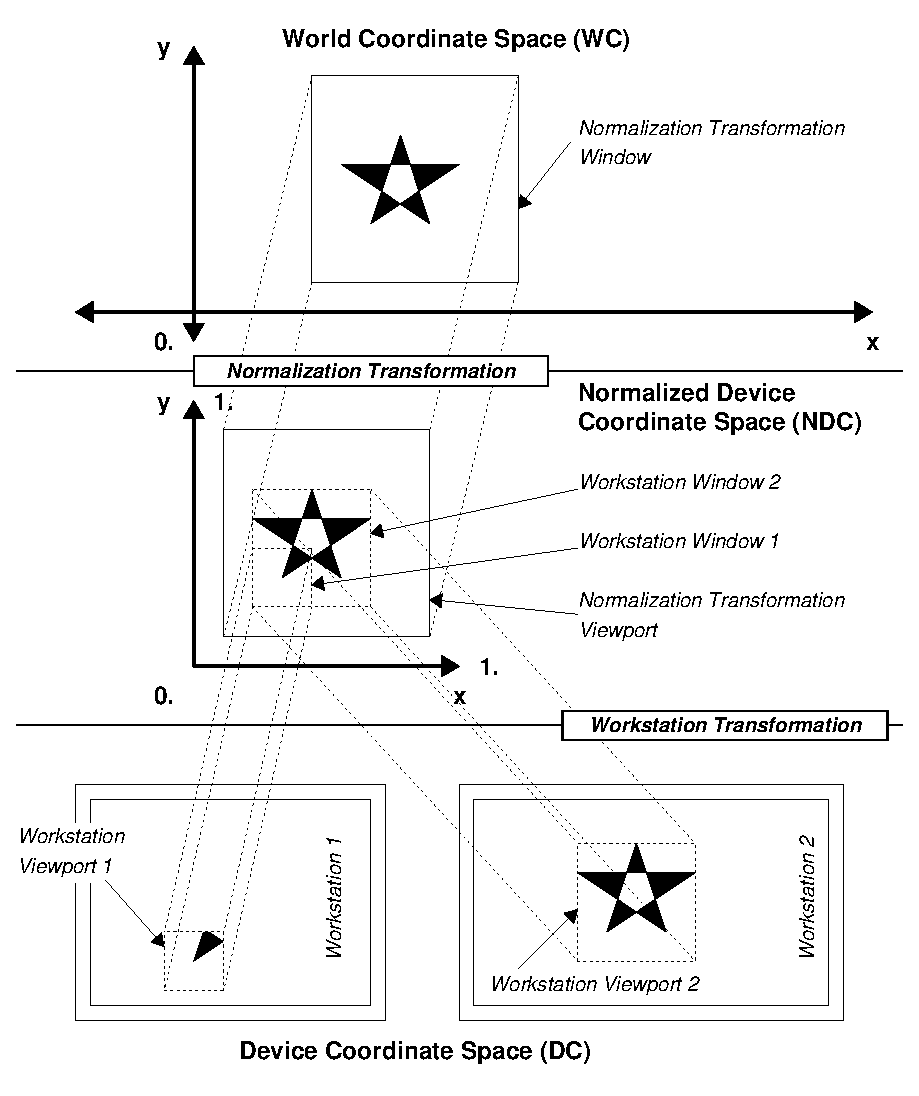
\includegraphics[width=\linewidth]{higznwt.eps}
\caption{Normalization and Workstation Transformations.}
\label{NTWT}
\end{figure}
\clearpage

\subsection{Workstation window definition}
\index{workstation!window definition}

\Shubr[GKS]{ISWKWN}{(KWKID,XMIN,XMAX,YMIN,YMAX)}
\Action
This routine defines a workstation window in the \NDC~space.
It sets the (requested) workstation window on a previously opened
workstation. The workstation window, specified in \NDC~
(i.e., {\tt0.-1.} by {\tt0.-1.}) is the portion of \NDC~space that the
application wishes to appear on the given workstation. This permits primitives
which are created when multiple workstations are active to be clipped and scaled
differently on the different workstations.

The workstation window (together with the workstation viewport and the rule that
the aspect ratio of the workstation window must be preserved) determines the
mapping (uniform scale with translation) from \NDC~to \DC.

The requested workstation window becomes the current workstation window either
during the invocation of \Rind{ISWKWN} (if the display surface is empty or if it
does not cause an implicit regeneration) or at some later time (for example,
during an invocation of \Rind{ICLRWK}).
\Pdesc
\begin{DLtt}{1234567}
\item[KWKID]Workstation identifier
\item[XMIN] X coordinate of the lower left hand corner in \ndc~space.
\item[XMAX] X coordinate of the upper right hand corner in \ndc~space.
\item[YMIN] Y coordinate of the lower left hand corner in \ndc~space.
\item[YMAX] Y coordinate of the upper right hand corner in \ndc~space.
\end{DLtt}
The four last parameters must be between {\tt0.0} and {\tt1.0}
(inclusive) and must satisfy {\tt XMIN < XMAX} and {\tt YMIN < YMAX}.
%
\subsection{Workstation viewport definition}
\index{workstation!viewport definition}
\Shubr[GKS]{ISWKVP}{(KWKID,XMIN,XMAX,YMIN,YMAX)}
\Action
This routine sets the (requested) workstation viewport on a previously opened
workstation. The workstation viewport, specified in \DC, is the
portion of the maximum available display surface that the application wishes to
use (see section \ref{IGQWK}).

The workstation viewport (together with the workstation window and the rule that
aspect ratios must be preserved) also determines the mapping (uniform scaling
with translation) from \NDC~to \DC.

The requested workstation viewport becomes the current workstation viewport
either during the invocation of \Rind{ISWKVP} (if the display surface is empty
or if it does not cause an implicit regeneration) or at some later time (for
example, during an invocation of \Rind{ICLRWK}). The \DC~region
specified by the parameters must be contained in  or equal to the maximum
available display  surface. The initial requested workstation viewport is the
entire display surface.
\Pdesc
\begin{DLtt}{1234567}
\item[KWKID]Workstation identifier
\item[XMIN] X coordinate of the lower left hand corner in \dc~space
\item[XMAX] X coordinate of the upper right hand corner in \dc~space
\item[YMIN] Y coordinate of the lower left hand corner in \dc~space
\item[YMAX] Y coordinate of the upper right hand corner in \dc~space
\end{DLtt}
The last four parameters must satisfy the conditions {\tt XMIN < XMAX} and
{\tt YMIN < YMAX}.
%
\subsection{Normalization Transformation window definition}
\index{normalization transformation!window definition}
\Shubr[GKS]{ISWN}{(NT,XMIN,XMAX,YMIN,YMAX)}
\Action
This routine sets the boundaries of the window of a \NT. The window must be
specified in \WC. The boundaries of the window, together with the
boundaries of the viewport (which are in \NDC)
determine a transformation from \WC~to \NDC~consisting of
separate X and Y scale factors and a translation in two dimensions. The \NT~is
selected by using routine \Rind{ISELNT}.
\Pdesc
\begin{DLtt}{1234567}
\item[NT]   Normalization transformation index ({\tt 0<NT<1000000}).
\item[XMIN] X coordinate of the lower left hand corner in \wc{} space.
\item[XMAX] X coordinate of the upper right hand corner in \wc{} space.
\item[YMIN] Y coordinate of the lower left hand corner in \wc{} space.
\item[YMAX] Y coordinate of the upper right hand corner in \wc{} space.
\end{DLtt}
The last four parameters must satisfy the conditions {\tt XMIN < XMAX} and
{\tt YMIN < YMAX}.
%
\subsection{Normalization Transformation viewport definition}
\index{normalization transformation!viewport definition}
\Shubr[GKS]{ISVP}{(NT,XMIN,XMAX,YMIN,YMAX)}
\Action
This routine sets the boundaries of the viewport of a \NT. The viewport must be
specified in \NDC. The boundaries of the viewport have
two roles:
\begin{OL}
\item Together with the boundaries of the window (which are in \WC)
      they determine a transformation from \WC~to \NDC~consisting of
      separate X and Y scale factors and a translation in two dimensions.
\item When the clipping indicator is 1 (see \Rind{ISCLIP}), primitives
      are clipped to the boundary of the viewport (once the primitives are
      transformed to \NDC)
\end{OL}
The \NT~is selected with the routine \Rind{ISELNT}.
\Pdesc
\begin{DLtt}{1234567}
\item[NT]   Normalization transformation index ({\tt 0<NT<1000000}).
\item[XMIN] X coordinate of the lower left hand corner in \ndc{} space
            ($0.0 \leq $\Lit{XMIN}$\leq 1.0$).
\item[XMAX] X coordinate of the upper right hand corner in \ndc{} space
            ($0.0 \leq $\Lit{XMAX}$\leq 1.0$).
\item[YMIN] Y coordinate of the lower left hand corner in \ndc{} space
            ($0.0 \leq $\Lit{YMIN}$\leq 1.0$).
\item[YMAX] Y coordinate of the upper right hand corner in \ndc{} space
            ($0.0 \leq $\Lit{YMAX}$\leq 1.0$).
\end{DLtt}
The last four parameters must satisfy the conditions {\tt XMIN < XMAX} and
{\tt YMIN < YMAX}.
%
\subsection{Normalization transformation selection}
\index{normalization transformation!selection}
\Shubr[GKS]{ISELNT}{(NT)}
\Action
This routine selects the \NT~to be used when \WC~must be mapped
to or from \NDC~(\ndc). These mappings usually take
place during invocations of primitives (\Rind{IFA}, \Rind{IPL}, \Rind{IPM}, and
\Rind{ITX}) and during graphics input (\Rind{IRQLC}).

Transformation {\tt0} always has a window and a viewport that are the unit
square ({\tt0.-1.} by {\tt0.-1.}) and cannot be changed with \Rind{ISVP} or
\Rind{ISWN}. Transformation {\tt0} is selected by default.
\Pdesc
\begin{DLtt}{1234567}
\item[NT] Normalization transformation index ({\tt 0<NT<1000000}). The number of transformations is
          limited to 50.
\end{DLtt}
%
\subsection{Simplified way to define the viewing pipeline}
\index{viewing pipeline}
Very often the user of a graphics package wants to define the dimensions of
the physical output in centimeters and centered on the output devices (screen or
paper). This can be done with \HIGZ~with simply one call to the routine
\Rind{IGRNG}.
\Shubr{IGRNG}{(XSIZE,YSIZE)}
\Action
\index{centimeter!to \NDC}
This routine is used to determine the physical dimensions (in centimeter)
and to optimize the aspect ratio and the centering of a picture.
If the {\tt X} or {\tt Y} dimension of output device are smaller than
{\tt XSIZE} or {\tt YSIZE}, a scaling factor is applied to the final size
of the picture but the aspect ratio is kept.
When an \EPS~workstation is active, a call to this routine is mandatory
in order to define the size of the picture (e.g the \PS~{\sf BoundingBox}).
\index{PostScript!Encapsulated!BoundingBox}
\Pdesc
\begin{DLtt}{1234567}
\item[XSIZE] Picture size in centimeters in the X direction.
\item[YSIZE] Picture size in centimeters in the Y direction.
\end{DLtt}
\par
After a call to \Rind{IGRNG} the \NT~number 1 is selected. For this reason
in all the \HIGZ~routines, the \NT~number {\tt 1} is assumed to be a centimeter
transformation. It is not recommended to define this transformation (via
\Rind{ISWN}, \Rind{ISVP} and \Rind{ISELNT}) outside \Rind{IGRNG}. In particular
when \PS~files are used, the \PS~driver assumes that the setting of the
\NT~{\tt 1} has been done via \Rind{IGRNG}.

After a call to \Rind{IGRNG} some useful value to convert centimeters into
\NDC{}, are available in the common \QUEST.
\begin{DLtt}{12345678901}
\item[RQUEST(11)] Ratio to convert cm into \NDC.
\item[RQUEST(12)] left position of the  \NT{} 1 viewport in \NDC.
\item[RQUEST(13)] bottom position of the \NT{} 1 viewport in \NDC.
\item[RQUEST(14)] width of the \NT{} 1 viewport in \NDC.
\item[RQUEST(15)] height of the \NT{} 1 viewport in \NDC.
\end{DLtt}
For more details, see examples on pages \pageref{HIEX1} and \pageref{HIEX4}.

\index{workstation!viewport definition}
\index{workstation!window definition}
%
%              Metafile control and printing
%

\section{Metafile control and printing}
\index{metafile!control}
\index{printing}
A special \ASCII~file called metafile is needed in order to produce pictures
on paper. The metafiles are managed via all workstation control routines
previously described. The general sequence of actions to use metafiles is:
\begin{verbatim}
- Open a FORTRAN file
- Open a workstation (IOPWK) with the type metafile
- Activate the workstation
- Produce some graphics
- Deactivate the workstation
- Close the workstation
\end{verbatim}
%
\subsection{Simplified metafile control}
The routine \Rind{IGMETA} is provided in order to minimize the number of
calls to specialized \HIGZ~workstation control routines and to improve
the portability of applications. This routine opens, activates, deactivates
or closes a metafile.

\Shubr{IGMETA}{(LUN,KWTYPE)}
\Action
This routine permits the selection of a metafile, offering a choice of graphic
output to the screen and/or a metafile.
\Pdesc
\begin{DLtt}{1234567}
\item[LUN] Metafile logical unit number
\begin{DLtt}{1234567}
\item[LUN>0] The subsequent graphic output will be directed to both screen and
             metafile.
\item[LUN<0] The subsequent graphic output will be directed to the metafile
             only.
\item[LUN=0] Any previously open metafile is deactivated, and further graphic
             output will be directed to the screen only.
\item[LUN=999] Any previously open metafile is deactivated and closed, and
               further graphic output will be directed to the screen only.
               \PS~metafiles need to be closed in order to be printed.
\end{DLtt}
\item[KWTYPE] Workstation type. If {\tt KWTYPE = 0}, then \Rind{IGMETA} selects
              automatically the default workstation type. This defaults
              workstations depend on the \UGP~used (e.g. -111 for
	      \HIGZ/\X11 or 4 for \GKSGRAL).
\end{DLtt}
%
\subsection{\PS~metafile type}
\index{metafile!PostScript}
In addition to the metafile type provided by the underlaying graphics
package (for example 4 with \GKSGRAL), \PS~workstation types
are also available independently from the \UGP~used allowing generation of
high quality outputs. The \PS~workstation types have the following format:
\begin{verbatim}
                               -[Format][Nx][Ny][Type]
\end{verbatim}
    Where:
\begin{DLtt}{1234567}
\item[Format] Is an integer between 0 and 99 which defines the format of the
              paper. \par
 Example: if {\tt Format}=3 the pa\-per is in the standard
	      A3 format. {\tt Format}=4 and {\tt Format}=0 are the same and
	      define an A4 page. The A0 format is selected by {\tt Format}=99.
              The US format Letter is selected by {\tt Format}=100.
              The US format Legal is selected by {\tt Format}=200.
              The US format Ledger is selected by {\tt Format}=300.
\item[Nx, Ny] Specify respectively the number of zones on the x and y axis.
              {\tt Nx} and {\tt Ny} are integers between 1 and 9.
\item[Type] Can be equal to:
\begin{DLtt}{12}
\item[1] Portrait mode with a small margin at the bottom of the page.
\item[2] Landscape mode with a small margin at the bottom of the page.
\item[4] Portrait mode with a large margin at the bottom of the page.
\item[5] Landscape mode with a large margin at the bottom of the page.

         The large
         margin is useful for some \PS~printers (very often for the colour
         printers) \index{PostScript!colour printers} as they need more space to
	 grip the paper for mechanical reasons.

         Note that some \PS~colour
	 printers can also use the so called "special A4" format permitting
	 the full usage of the A4 area; \index{PostScript!special A4} in this
	 case larger margins are not necessary and {\tt Type}=1 or 2
         can be used.
\item[3] \EPS. This {\tt Type} permits the generation of files which can be
         included in other documents, for example \index{latex@\LaTeX{}!PostScript}
         in \LaTeX{} files. Note that with this {\tt Type}, {\tt Nx} and
	 {\tt Ny} must always be equal to 1, and {\tt Format} has no meaning.
	 The size of the picture must be specified by the user via the
	 \Rind{IGRNG} routine. Therefore the workstation type for \EPS~is -113.
	 For example if the name of an \EPS~file is {\tt example.eps}, the
	 inclusion of this file into a \LaTeX{} file will be possible via
	 (in the \LaTeX{} file):
\begin{verbatim}
   \begin{figure}
   \includegraphics{example.eps}
   \caption{Example of Encapsulated PostScript in LaTeX.}
   \label{EXAMPLE}
   \end{figure}
\end{verbatim}
Note that all the figures in this manual are included in this way.
\end{DLtt}
\end{DLtt}
With {\tt Type=1,2,4} and 5 the pictures are centered on the page, and the
usable area on paper is proportional to the dimensions of A4 format.
\par
Examples:
\par
\Lit{-111} or \Lit{-4111} defines an A4 page not divided.
\Lit{-6322} define an A6 landscape page divided in 3 columns and 2 rows.
\begin{center}
\extrarowheight=1mm
\begin{tabular}{|*{3}{>{\quad}c<{\quad}|}}
\hline
1 & 2 & 3 \\ \hline
4 & 5 & 6 \\ \hline
\end{tabular}
\end{center}
The first picture  will be drawn  in the area 1. If the program clears the
screen via \Rind{ICLRWK}, the graphics output will appear in  the next area in
the order defined above. If a  page is filled, a new  page is used with
the same grid. Note that empty  pages are not printed  in order to save
paper.
\par
Ignoring  formats smaller  than A12, the total number of possible different
\PS~workstation types is: $4\times9\times9\times13+1 = 4213$ !

\subsection{Usage of \PS~metafiles in an user application program}
This section gives three examples showing the different ways of managing
\PS~files. The first example is the more general way, using
\Rind{IOPWK}, \Rind{IACWK} and \Rind{IGQWK} (see section \ref{IGQWK}). The
second example shows how to use the \Rind{IGMETA} routine. The last example
use \Rind{IGRNG} and \Rind{IGMETA}.
\begin{XMPt}{Example 1 : \Rind{IOPWK}, \Rind{IACWK} and \Rind{IGQWK}}

      DIMENSION R(2)
*
*              Open a \FORTRAN file. Note that on VAX/VMS machines
*              a CARRIAGECONTROL='LIST' in the open statement is needed.
*
      OPEN(UNIT=10,FILE='test1.ps',FORM='FORMATTED',STATUS='UNKNOWN')
*
*              Open and activate a workstation with the \PS metafile
*              type -111 and with the workstation ID 5.
*              Note that the UNIT used to open the \FORTRAN (here 10)
*              is given as second parameter.
*
      CALL IOPWK(5,10,-111)
      CALL IACWK(5)
*
*              Get the size of the available space on paper. This is
*              now possible because the Format is known.
*
      CALL IGQWK(5,'MXDS',R)
*
*              Compute the size of the viewport according to the paper
*              size. Note that if the screen has not the same RATIO the
*              picture on screen and on paper will be different. In this
*              case the user must inquire the screen size and compute
*              a new viewport with this size and redraw on the screen
*              with the metafile deactivated.
*
      XV=R(1)/R(2)/2.
      YV=XV
      CALL ISVP(2,0.,XV,0.,YV)
      CALL ISWN(2,X1,X2,Y1,Y2)
      CALL ISELNT(2)
          .
          .
        Drawing
          .
          .
*
*              Deactivate and close the metafile
*
      CALL IDAWK(5)
      CALL ICLWK(5)
      CLOSE(10)

\end{XMPt}
\begin{XMPt}{Example 2 : \Rind{IGMETA}}

      DIMENSION R(2)
      OPEN(UNIT=10,FILE='test2.ps',FORM='FORMATTED',STATUS='UNKNOWN')
*
*              IGMETA permits the opening and activating of the metafile
*
      CALL IGMETA(10,-111)
      CALL IGQWK(2,'MXDS',R)
      XV=MIN(1.,R(1)/R(2))
      YV=MIN(1.,R(2)/R(1))
      CALL ISVP(2,0.,XV,0.,YV)
      CALL ISWN(2,X1,X2,Y1,Y2)
      CALL ISELNT(2)
          .
          .
        Drawing
          .
          .
*
*              Deactivate the metafile
*
      CALL IGMETA(0,0)
*
*              Close the metafile
*
      CALL ICLWK(2)
      CLOSE(10)

\end{XMPt}
\begin{XMPt}{Example 3 : \Rind{IGRNG}}

      DIMENSION R(2)
      OPEN(UNIT=10,FILE='test4.ps',FORM='FORMATTED',STATUS='UNKNOWN')
      CALL IGMETA(-10,-111)
*
*              IGRNG defines a size in cm centered on the page.
*              Even if the RATIO of the screen and the RATIO of
*              the paper are not the same the picture will appear
*              exactly the same on both.
*              Note that in the case of \EPS~(-113)
*              a call to IGRNG is mandatory.
*
      CALL IGRNG(10.,10.)
          .
          .
        Drawing
          .
          .
      CALL IGMETA(0,0)
      CALL ICLWK(2)
      CLOSE(10)
\end{XMPt}
\subsection{\LaTeX{} metafile type}
\index{metafile!\LaTeX{}}
\index{latex@\LaTeX{}}
\HIGZ~is able to produce metafiles which are ready to be included in \LaTeX{}
documents. These metafiles make use of the \verb'\picture' environment.
Compared to other possibilities of merging graphics
into documents, \LaTeX{} metafiles have a number of advantages:

\begin{ULc}
\item  The {\tt dvi} file is fully transportable as \verb'\special' commands are
       not used. This file can be output on any device for which a driver
       exists. Documents can be written, formatted, and previewed on
       workstations while the {\tt dvi} file can be sent via the  network to a
       central server for printing.
\item  The metafile can be also merged into the \LaTeX{} file to keep
       the full document in a single file.
\item  The power of \LaTeX{} in text processing can be used in the primitive
       \Rind{ITX} for example to generate complicated mathematical formulae
       on a document.
\end{ULc}

\subsubsection{\LaTeX{} metafile capabilities}

The capabilities of the \verb'\picture' environment are basically limited to
drawing straight horizontal or vertical lines. Slanted lines do exist but only
in a limited number of slopes and a minimum length of $\approx 4 {\rm mm}$.
Therefore slanted lines have to be approximated by small steps of straight lines
where the step size should be close to the printer resolution.
\par
The workstation type for \LaTeX{} metafiles is -777 for embedded files or
-778 for stand-alone files. Coordinates written to the metafile are integer
numbers assuming a grid spacing of $0.1 {\rm mm}$. Therefore the settings for
{\tt XSIZE} and {\tt YSIZE} should approximately correspond to the final
picture size.

\subsubsection{Line and marker types}

Line types 1 through 4 and marker types 1 through 5 are supported.

\subsubsection{Text fonts}

In addition to the software characters the font numbers -1 through -8 at
precision 0 can
be used. They map to the \TeX{} fonts {\rm Roman}, {\em Emphatic}, {\bf Bold},
{\it Italic}, {\sl Slanted}, {\sf Sans Serif}, {\sc Small Caps}, and
{\tt Typewriter}, respectively.
\par
\TeX{} fonts look much nicer and are faster to generate than software
characters generated by \Rind{IGTEXT}, but the disadvantage is that they are
available in horizontal orientation only and the character size does not scale
with the picture size.
\par
When using \TeX{} fonts the \Rind{IGTEXT} control characters
``\verb'<>[]"#^?!''' are interpreted to obtain superscripts, greek letters, and
other special characters. If a text string contains a ``\verb'\''' or
``\verb'{''' the remaining part is written verbatim into the metafile.
This allows to use \TeX{} formatting commands for elaborate displays.
Of course ``\verb'{''' and ``\verb'}''' must be properly matched.
\par
The whole text is typeset in math mode which does not allow a change of
fontsize in between. In order to format a formula on a larger size the formula
text must be preceded by ``\verb'{}$\large$'''.
\par
%\subsubsection{Example}
%\begin{figure}
%% HIGZ version 1.13/06 LaTeX metafile created  91/11/04   12.46
\ifx\higzunit\undefined\unitlength=0pt{}\else\unitlength=\higzunit\fi\ifdim\unitlength=0pt\unitlength=\textwidth\divide\unitlength
 2000\fi\par\noindent\begin{picture}(2000,2000)(0,0)\ifx\higzdraft\undefined\newcount\higzdraft\higzdraft=0{}\fi\ifnum\higzdraft>0
\put(0,0){\framebox(2000,2000){}}\else\ifx\higzstep\undefined\newcount\higzstep\higzstep=0{}\fi\ifnum\higzstep<1\higzstep=2
\fi\ifx\higzxx\undefined\newcount\higzxx\newcount\higzyy\newcount\higzx\newcount\higzy\newcount\higzdx\newcount\higzdy
\newcount\higzlx\newcount\higzly\newcount\higzslope\newcount\higzlen\newcount\higzllen\newcount\higzoffs\newcount\higzloffs
\newcount\higzadash\newcount\higzbdash\newcount\higzcdash\newcount\higzddash\newcount\higzmsize\newcount\higztemp\fi
\def\higzstroke#1,#2,#3,#4;{\advance\higzloffs\higzllen\ifnum\higzloffs>#1\advance\higzloffs-\higzllen\advance\higzloffs-#1
\higzloffs=-\higzloffs\ifnum#2>0\put(\higzlx,\higzly){\line(#3,#4){\higzloffs}}\fi\ifnum#2<0\put(\higzlx,\higzly){\circle*{0}}\fi
\higztemp=\higzloffs\multiply\higztemp#3\advance\higzlx\higztemp\higztemp=\higzloffs\multiply\higztemp#4\advance\higzly\higztemp
\advance\higzllen-\higzloffs\higzloffs=#1\else\ifnum#2>0\put(\higzlx,\higzly){\line(#3,#4){\higzllen}}\fi\ifnum#2<0\put(
\higzlx,\higzly){\circle*{0}}\fi\higzllen=0\fi}\def\higzdashed#1,#2,#3,#4,#5;{{\higzlx=#1\higzly=#2\higzllen=#5\higzloffs=
\higzoffs\loop\ifnum\higzloffs<\higzadash\ifnum\higzadash>1\higzstroke\higzadash,1,#3,#4;\else\higzstroke\higzadash,-1,#3,#4;\fi
\else\ifnum\higzloffs<\higzbdash\higzstroke\higzbdash,0,#3,#4;\else\ifnum\higzloffs<\higzcdash\higztemp=\higzcdash\advance
\higztemp-\higzbdash\ifnum\higztemp>1\higzstroke\higzcdash,1,#3,#4;\else\higzstroke\higzcdash,-1,#3,#4;\fi\else\ifnum\higzloffs<
\higzddash\higzstroke\higzddash,0,#3,#4;\else\higzloffs=0\fi\fi\fi\fi\ifnum\higzllen>0\repeat\global\higzoffs=\higzloffs}}\def
\higzsolid#1,#2,#3,#4,#5;{\put(#1,#2){\line(#3,#4){#5}}}\def\higzhslant#1,#2,#3;{\higzslope=#1\multiply\higzslope1000\advance
\higzslope500\divide\higzslope#2\higzlen=\higzslope\multiply\higzlen\higzstep\divide\higzlen1000\higzdy=0\loop\ifnum
\higzdy<#2\higzx=\higzxx\higzy=\higzyy\higzdx=\higzslope\multiply\higzdx\higzdy\advance\higzdx500\divide\higzdx1000\advance
\higzy\higzdy\multiply\higzdx#3\advance\higzx\higzdx\multiply\higzdx#3\advance\higzdx\higzlen\ifnum\higzdx>#1\advance
\higzlen#1\advance\higzlen-\higzdx\fi\higzline\higzx,\higzy,#3,0,\higzlen;\advance\higzdy\higzstep\repeat}\def\higzvslant#1,#2,#3;{
\higzslope=#2\multiply\higzslope1000\advance\higzslope500\divide\higzslope#1\higzlen=\higzslope\multiply\higzlen\higzstep
\divide\higzlen1000\higzdx=0\loop\ifnum\higzdx<#1\higzx=\higzxx\higzy=\higzyy\higzdy=\higzslope\multiply\higzdy\higzdx\advance
\higzdy500\divide\higzdy1000\advance\higzx\higzdx\multiply\higzdy#3\advance\higzy\higzdy\multiply\higzdy#3\advance
\higzdy\higzlen\ifnum\higzdy>#2\advance\higzlen#2\advance\higzlen-\higzdy\fi\higzline\higzx,\higzy,0,#3,\higzlen;\advance\higzdx
\higzstep\repeat}\def\s#1,#2;{\higzdx=#1{}\ifnum\higzdx<0\higzdx=-\higzdx\fi\higzdy=#2{}\ifnum\higzdy<0\higzdy=-\higzdy\fi\ifnum
\higzdx<\higzdy\ifnum#1<0\advance\higzxx#1\advance\higzyy#2\ifnum#2<0\higzvslant-#1,-#2,1;\else\higzvslant-#1,#2,-1;
\fi\else\ifnum#2<0\higzvslant#1,-#2,-1;\else\higzvslant#1,#2,1;\fi\advance\higzxx#1\advance\higzyy#2\fi\else\ifnum#2<0
\advance\higzxx#1\advance\higzyy#2\ifnum#1<0\higzhslant-#1,-#2,1;\else\higzhslant#1,-#2,-1;\fi\else\ifnum#1<0
\higzhslant-#1,#2,-1;\else\higzhslant#1,#2,1;\fi\advance\higzxx#1\advance\higzyy#2\fi\fi}\def\h#1;{\higzline\higzxx,
\higzyy,1,0,#1;\advance\higzxx#1}\def\r#1;{\higzline\higzxx,\higzyy,-1,0,#1;\advance\higzxx-#1}\def\U#1;{\higzline\higzxx,
\higzyy,0,1,#1;\advance\higzyy#1}\def\D#1;{\higzline\higzxx,\higzyy,0,-1,#1;\advance\higzyy-#1}\def\m#1,#2;{\higzxx=#1
\higzyy=#2}\def\higzdot#1,#2;{\put(#1,#2){\circle*{\higzmsize}}}\def\higzplus#1,#2;{\higzx=#1\multiply\higzx2\advance\higzx-
\higzmsize\divide\higzx2\put(\higzx,#2){\line(1,0){\higzmsize}}\higzy=#2\multiply\higzy2\advance\higzy-\higzmsize\divide
\higzy2\put(#1,\higzy){\line(0,1){\higzmsize}}}\def\higzstar#1,#2;{\higzplus#1,#2;\higzcross#1,#2;}\def
\higzcircle#1,#2;{\put(#1,#2){\circle{\higzmsize}}}\def\higzcross#1,#2;{\let\higzsave\higzline\let\higzline\higzsolid\higzlx=#1
\multiply\higzlx2\advance\higzlx-\higzmsize\divide\higzlx2\higzly=#2\multiply\higzly2\advance\higzly-\higzmsize\divide
\higzly2\m\higzlx,\higzly;\s\higzmsize,\higzmsize;\higzly=#2\multiply\higzly2\advance\higzly\higzmsize\divide\higzly2\m\higzlx,
\higzly;\s\higzmsize,-\higzmsize;\let\higzline\higzsave}\def\p#1,#2;{\higzmarker#1,#2;}\def\f#1,#2;{\put(\higzxx,
\higzyy){\makebox(#1,#2)[lb]{\rule{#1\unitlength}{#2\unitlength}}}}
% End of Initialisation
\let\higzline=\higzsolid\put(0,0){\framebox(2268,2268){}}\put(227,227){\framebox(1814,1814){}}\put(2211,2177){\makebox(0,0)[br]
{$\sf{}91/11/04\ {}\ {}\ {}12.46$}}
\fi\end{picture}

%\end{figure}

\subsubsection{Configuration parameters}
To some extent, the appearance of a picture can be changed at formatting time
by defining configuration parameters (in the \LaTeX{} file) which have the
following default values:
\begin{verbatim}
\newdimen\higzunit \higzunit=0pt
\newcount\higzstep \higzstep=2
\newcount\higzdraft \higzdraft=0
\end{verbatim}
\par
\index{higzunit}
By default the picture is automatically scaled to fill the full page width.
The picture size can be changed by setting \verb'\higzunit' to the wanted grid
spacing, e.g. to get the true {\tt XSIZE}:
\begin{verbatim}
\newdimen\higzunit \higzunit=0.1mm
\end{verbatim}
\par
\index{higzstep}
Slanted lines are approximated by straight lines along the major axis.
The step size along the minor axis is
\verb'\higzstep'$\times$\verb'\unitlength'.
By setting \verb'\higzstep=1' curves will look smoother
but if line segments come too close to the printer resolution the
{\tt dvi} driver may choose not to display them.
A larger value will result in faster formatting requiring less \TeX{} memory.
\par
\index{higzdraft}
Setting \verb'\higzdraft=1' replaces the actual picture by an empty box
of the same size to save formatting time during drafting.
%

\section{Examples: the routines {\tt START} and {\tt FINISH}}
The two routines used to produce the figures appearing this manual are
described in this section. They are good examples of a simple, but frequent,
usage of \HIGZ.

The first one: {\tt START}, initializes \HIGZ, opens an \EPS~file and set the
size of the figure according to the input parameters.

The second one: {\tt FINISH}, closes the \EPS~file and terminates \HIGZ.

\begin{XMPt}{The routine {\tt START}}
      SUBROUTINE START(NAME,X,Y)
      CHARACTER*(*) NAME
      PARAMETER (NWORDS=50000)
      COMMON /PAWC/ RPAW(NWORDS)
      CALL MZEBRA(-3)
      CALL MZPAW(NWORDS,' ')
      CALL IGINIT(0)
      CALL IGWKTY(ITYPE)
      CALL IGSSE(6,ITYPE)
      OPEN(UNIT=10,FILE=NAME//'.EPS',FORM='FORMATTED',STATUS='UNKNOWN')
      CALL IGMETA(10,-113)
      CALL IGRNG(X,Y)
      END
\end{XMPt}
In the routine {\tt FINISH} the call to the routine {\tt IGTERM} is not
mandatory but is useful to flush the graphics buffer especially in the
case of the \X11~interface (see section \ref{IGTERM}).
\begin{XMPt}{The routine {\tt FINISH}}
      SUBROUTINE FINISH
      CALL IGMETA(999,0)
      CLOSE(10)
      CALL IGTERM
      CALL IGEND
      END
\end{XMPt}
\newpage
%
%              The basic output primitives
%

\section{The basic output primitives}
\index{primitives}
\par
In \HIGZ~there are four basic output primitives: the polyline (\Rind{IPL}),
the fill area (\Rind{IFA}), the polymarker (\Rind{IPM}) and the text
(\Rind{ITX}). In all routines described in this section the coordinates
are given in the \WC~system.


\subsection{Polyline}
\index{primitives!polyline}
\index{polyline!drawing}
\Shubr[GKS]{IPL}{(N,X,Y)}
\Action
This routine draws a polyline on the currently active workstations (there must
be at least one). The polyline connects {\tt N} points ({\tt N$\geq$2}) by means
of {\tt N-1} line segments. The {\tt X} and {\tt Y} coordinates of the points
are in two {\tt N}-dimensional arrays.

The appearance of a polyline is controlled by the current ``polyline colour
index'' (see \Rind{ISPLCI} section \ref{ISPLCI}), the current
``line type'' (see \Rind{ISLN} section \ref{ISLN}) and the current
``line width'' (see \Rind{ISLWSC} section \ref{ISLWSC}).
\Pdesc
\begin{DLtt}{1234567}
\item[N] Number of points.
\item[X] Array of dimension {\tt N} containing the x coordinates in \wc~space.
\item[Y] Array of dimension {\tt N} containing the y coordinates in \wc~space.
\end{DLtt}


\subsection{Multiline}
\index{primitives!Multiline}
\index{Multiline!drawing}
\Shubr{IML}{(N,X,Y)}
\Action
This routine draws a multiline on the currently active workstations (there must
be at least one). The multiline connects \Lit{N} points ({\tt N$\geq$2}) two
by two. The \Lit{X} and \Lit{Y} coordinates of the points are in two 
\Lit{N}-dimensional arrays.

The appearance of a multiline is controlled by the current ``polyline colour
index'' (see \Rind{ISPLCI} section \ref{ISPLCI}), the current
``line type'' (see \Rind{ISLN} section \ref{ISLN}) and the current
``line width'' (see \Rind{ISLWSC} section \ref{ISLWSC}).
\Pdesc
\begin{DLtt}{1234567}
\item[N] Number of points.
\item[X] Array of dimension {\tt N} containing the x coordinates in \wc~space.
\item[Y] Array of dimension {\tt N} containing the y coordinates in \wc~space.
\end{DLtt}

\newpage

\subsection{Polymarker}
\index{primitives!polymarker}
\index{polymarker!drawing}
\Shubr[GKS]{IPM}{(N,X,Y)}
\Action
This routine draws a polymarker on the currently active workstations (there must
be at least one). Markers are placed at {\tt N} points ({\tt N$\geq$1}), whose x
and y coordinates are given in two {\tt N}-dimensional arrays.

The appearance of a polymarker is controlled by the current ``polymarker colour
index'' (see \Rind{ISPMCI} section \ref{ISPMCI}), the current ``marker
type'' (see \Rind{ISMK} section \ref{ISMK}) and the current ``marker
scale factor'' (see \Rind{ISMKSC} section \ref{ISMKSC}).
\Pdesc
\begin{DLtt}{1234567}
\item[N] Number of points.
\item[X] Array of dimension {\tt N} containing the x coordinates in \wc~space.
\item[Y] Array of dimension {\tt N} containing the y coordinates in \wc~space.
\end{DLtt}


\subsection{Fill area}
\index{primitives!fill area}
\index{fill area!drawing}
\Shubr[GKS]{IFA}{(N,X,Y)}
\Action
This routine draws a filled area on the currently active workstations (there
must be at least one). The ``perimeter'' of the filled area has {\tt N} points
({\tt N$\geq$3}) whose x and y coordinates are given in two {\tt N}-dimensional
arrays.

The appearance of a filled area is controlled by the current ``filled area
colour index'' (see \Rind{ISFACI} section \ref{ISFACI}), the current
``filled area interior style'' (see \Rind{ISFAIS} section \ref{ISFAIS})
and the current ``filled area style index'' (see \Rind{ISFASI} section
\ref{ISFAIS}).
\Pdesc
\begin{DLtt}{1234567}
\item[N] Number of points.
\item[X] Array of dimension {\tt N} containing the x coordinates in \wc~space.
\item[Y] Array of dimension {\tt N} containing the y coordinates in \wc~space.
\end{DLtt}
%
\subsection{Text}
\index{primitives!text}
\index{text!drawing}
\Shubr[GKS]{ITX}{(X,Y,CHARS)}
\Action
This routine draws a text string on the currently active workstations
(there must be at least one).

The appearance of the text is controlled by attributes set by the current ``text
colour index'' (see \Rind{ISTXCI} section \ref{ISTXCI}), the current
``character height'' (see \Rind{ISCHH} section \ref{ISCHH}), the current
``text orientation'' (see \Rind{ISCHUP} section \ref{ISCHUP} and the
option {\tt TANG} of the routine \Rind{IGSET} section \ref{IGSET}), the current
``text alignment'' (see \Rind{ISTXAL} section \ref{ISTXAL}) and the
current ``text font and precision'' (see \Rind{ISTXFP} section
\ref{ISTXFP}).
\Pdesc
\begin{DLtt}{1234567}
\item[X] X coordinate in \wc~space.
\item[Y] Y coordinate in \wc~space.
\item[CHARS] {\tt CHARACTER} variable containing the text to be displayed.
             Only the following characters are allowed to appear in {\tt CHARS}:
\begin{verbatim}
     !"#\$%&'()*+,-./0123456789:;<=>?
     @ABCDEFGHIJKLMNOPQRSTUVWXYZ[-]^_
     abcdefghijklmnopqrstuvwxyz{|}~
     and the space.
\end{verbatim}
\end{DLtt}
Software characters (i.e. drawn with lines and not provided by the hardware) can
be produced with routine \Rind{IGTEXT}.
\index{text!software}
\index{text!hardware}
%
%              The output attributes
%

\section{The output attributes}
\index{primitives!attributes}
%
\subsection{Clipping}
\index{clipping}
\Shubr[GKS]{ISCLIP}{(ICLSW)}
\Action
This routine sets the ``clipping indicator'' for use by future invocations of
\Rind{IFA}, \Rind{IPL}, \Rind{IPM} and \Rind{ITX}. The clipping indicator
specifies where primitives should be clipped.
\Pdesc
\begin{DLtt}{1234567}
\item[ICLSW] Clipping indicator
\begin{DLtt}{123}
\item[1] Primitives should be clipped at the boundary of the \NT~viewport.
\item[0] Primitives should be clipped at the edge of the \NDC~space.
\end{DLtt}
\end{DLtt}
%
%
%
\subsection{Colour management}
\index{colour}
\subsubsection{Colour representation}
Each colour is defined by an index and percentages of red, green and blue.
Once a colour is defined it can be used via a reference to its index. If a
requested colour index is not available on a workstation, colour index {\tt 1}
is used when primitives are created.
\index{colour!representation}
\Shubr[GKS]{ISCR}{(KWKID,ICI,CR,CG,CB)}
\Action
This routine sets the colour representation (red/green/blue) of the colour index
on a previously opened workstation. On workstations using colour tables, this
function can change the image immediately. On workstations lacking such tables,
this new colour definition will be taken into account in the next use of this
colour.
\Pdesc
\begin{DLtt}{1234567}
\item[KWKID] Workstation identifier
\item[ICI]   Colour index.
\item[CR]    Intensity of red {\tt0.$\leq$CR$\leq$1.}
\item[CG]    Intensity of green {\tt0.$\leq$CG$\leq$1.}
\item[CB]    Intensity of blue {\tt0.$\leq$CB$\leq$1.}
\end{DLtt}
By default \Rind{IGSSE} initialize the first eight colour indices are defined as follows:
\begin{center}
\begin{tabular}{||c|l|c|c|c||}
\hline
Index & Colour & Red & Green & Blue \\
\hline
0 & Background colour (White) & 1. & 1. & 1. \\
1 & Foreground colour (Black) & 0. & 0. & 0. \\
2 & Red                       & 1. & 1. & 1. \\
3 & Green                     & 0. & 1. & 0. \\
4 & Dark blue                 & 0. & 0. & 1. \\
5 & Yellow                    & 1. & 1. & 0. \\
6 & Magenta (red-purple)      & 1. & 0. & 1. \\
7 & Cyan (light blue)         & 0. & 1. & 1. \\
\hline
\end{tabular}
\end{center}
%
\index{PostScript!colour emulation}
When a \PS~file is printed on a black and white \PS~printer, a grey level
simulation of the colours is used according to the
figure \ref{COLPS}.
\begin{figure}[t]
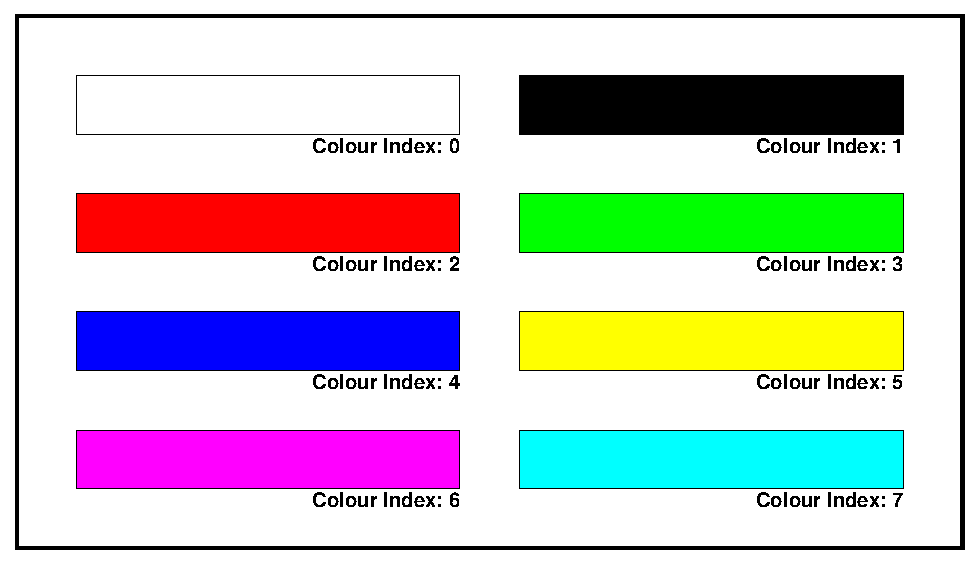
\includegraphics{col8.eps}
\caption{\PS~grey level simulation of the eight basic colours.}
\label{COLPS}
\end{figure}
%
\subsubsection{Polyline colour index.}
\index{polyline!colour index}
\index{colour!polyline}
\Shubr[GKS]{ISPLCI}{(ICOLI)}
\Action
This routine sets the polyline colour index attribute for use by future
invocations of \Rind{IPL}. The routine \Rind{IGSET} (see section \ref{IGSET})
can also be used with the parameter \Sind{PLCI}.
\Pdesc
\begin{DLtt}{1234567}
\item[ICOLI] Polyline colour index.
\end{DLtt}
%
\subsubsection{Polymarker colour index.}
\index{polymarker!colour index}
\index{colour!polymarker}
\Shubr[GKS]{ISPMCI}{(ICOLI)}
\Action
This routine sets the polymarker colour index attribute for use by future
invocations of \Rind{IPM}. The routine \Rind{IGSET} (see section \ref{IGSET})
can also be used with the parameter \Sind{PMCI}.
\Pdesc
\begin{DLtt}{1234567}
\item[ICOLI] Polymarker colour index.
\end{DLtt}
%
\subsubsection{Fill area colour index.}
\index{fill area!colour index}
\index{colour!fill area}
\Shubr[GKS]{ISFACI}{(ICOLI)}
\Action
This routine sets the fill area colour index attribute for use by future
invocations of \Rind{IFA}. The routine \Rind{IGSET} (see section \ref{IGSET})
can also be used with the parameter \Sind{FACI}.
\Pdesc
\begin{DLtt}{1234567}
\item[ICOLI] Fill area colour index.
\end{DLtt}
%
\clearpage
\subsubsection{Text colour index.}
\index{text!colour index}
\index{colour!text}
\Shubr[GKS]{ISTXCI}{(ICOLI)}
\Action
This routine sets the text colour index attribute for use by future invocations
of \Rind{ITX}. The routine \Rind{IGSET} (see section \ref{IGSET}) can also be
used with the parameter \Sind{TXCI}.
\Pdesc
\begin{DLtt}{1234567}
\item[ICOLI]Text colour index.
\end{DLtt}
%
\subsection{Fill area interior style}
\index{fill area!interior style}
\Shubr[GKS]{ISFAIS}{(INTS)}
\Action
This routine sets the fill area interior style attribute for use by future
invocations of \Rind{IFA}. The routine \Rind{IGSET} (see section \ref{IGSET})
can also be used with the parameter \Sind{FAIS}.
\Pdesc
\begin{DLtt}{1234567}
\item[INTS] Fill area interior style. Possible values are:
\begin{DLtt}{123}
\item[0] Hollow: the perimeter of the filled area, after clipping, is drawn
         using solid lines.
\item[1] Solid: the area is filled solidly.
\item[2] Pattern: the area is filled with a dot-dashed pattern.
\item[3] Hatched: the area is filled according to the current
value of the fill area style index.
\end{DLtt}
\end{DLtt}
\begin{Fighere}
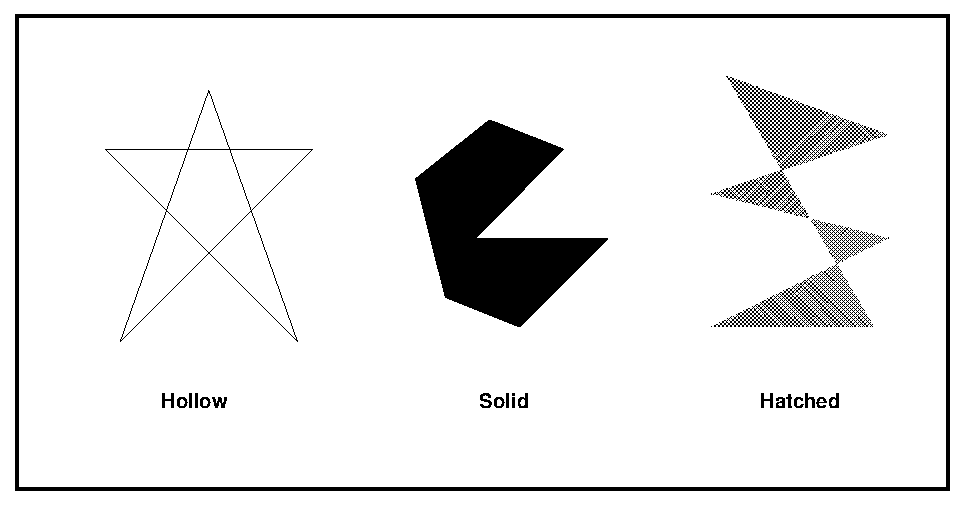
\includegraphics[width=\linewidth]{fais.eps}
\caption{Example of fill area interior style.}
\label{FILL-IS}
\end{Fighere}
%
\newpage
\subsection{Fill area style index.}
\index{fill area!style index}
\Shubr[GKS]{ISFASI}{(ISTYLI)}
\Action
This routine sets the fill area style index for pattern and hatch styles. The
routine \Rind{IGSET} (see section \ref{IGSET}) can also be used with the
parameter \Sind{FASI}.
\Pdesc
\begin{DLtt}{1234567}
\item[ISTYLI] Fill area style index. This value depends on the \UGP~used.
\end{DLtt}
In addition to the \UGP~dependent Fill area style indices, \HIGZ~provides a set
of hatches independent from the \UGP~used. This fill area styles are indicated
by a value greater than 100. The fill area style index is coded on three digits
{\tt ijk}.
\begin{DLtt}{1234567}
\item[i] Distance between lines in the hatch.
\item[j] Angle between 90 and 180 degrees.
\item[k] Angle between  0 and  90 degrees.
\end{DLtt}
\begin{center}
\begin{tabular}{||c|c||c|c||c|c||}
\hline
Digit i  &      Distance      &  Digit j  &  Angle  &   Digit k  &  Angle  \\
\hline
         &                    &     0     & 180 deg &     0      &   0 deg \\
  1      & $\approx$ 0.75 mm  &     1     & 170 deg &     1      &  10 deg \\
  2      & $\approx$ 1.50 mm  &     2     & 160 deg &     2      &  20 deg \\
  3      & $\approx$ 2.25 mm  &     3     & 150 deg &     3      &  30 deg \\
  4      & $\approx$ 3.00 mm  &     4     & 135 deg &     4      &  45 deg \\
  5      & $\approx$ 3.75 mm  &     5     &not drawn&     5      &not drawn\\
  6      & $\approx$ 4.50 mm  &     6     & 120 deg &     6      &  60 deg \\
  7      & $\approx$ 5.25 mm  &     7     & 110 deg &     7      &  70 deg \\
  8      & $\approx$ 6.00 mm  &     8     & 100 deg &     8      &  80 deg \\
  9      & $\approx$ 6.75 mm  &     9     &  90 deg &     9      &  90 deg \\
\hline
\end{tabular}
\end{center}
For example {\tt 190} will set the interior of fill areas to be hatched with
lines at 0 and 90 degrees ($\approx$ 0.75 mm spacing) and {\tt 444} will set
the interior of fill areas to be hatched with lines at +45 and -45 degrees
($\approx$ 3 mm spacing).

The figure \ref{FILL-STY} shows some examples of \HIGZ~portable hatch styles.
On this figure, the first column shows the nine different possible spacing
(digit {\tt i}), the second column shows the angle between {\tt 90} and
{\tt 180} degrees (digit {\tt j}), and the third column shows the angle between
{\tt 0} and {\tt 90} degrees (digit {\tt k}).

The number of possible hatch styles is: $9\times10\times10=900$.
\begin{figure}[p]
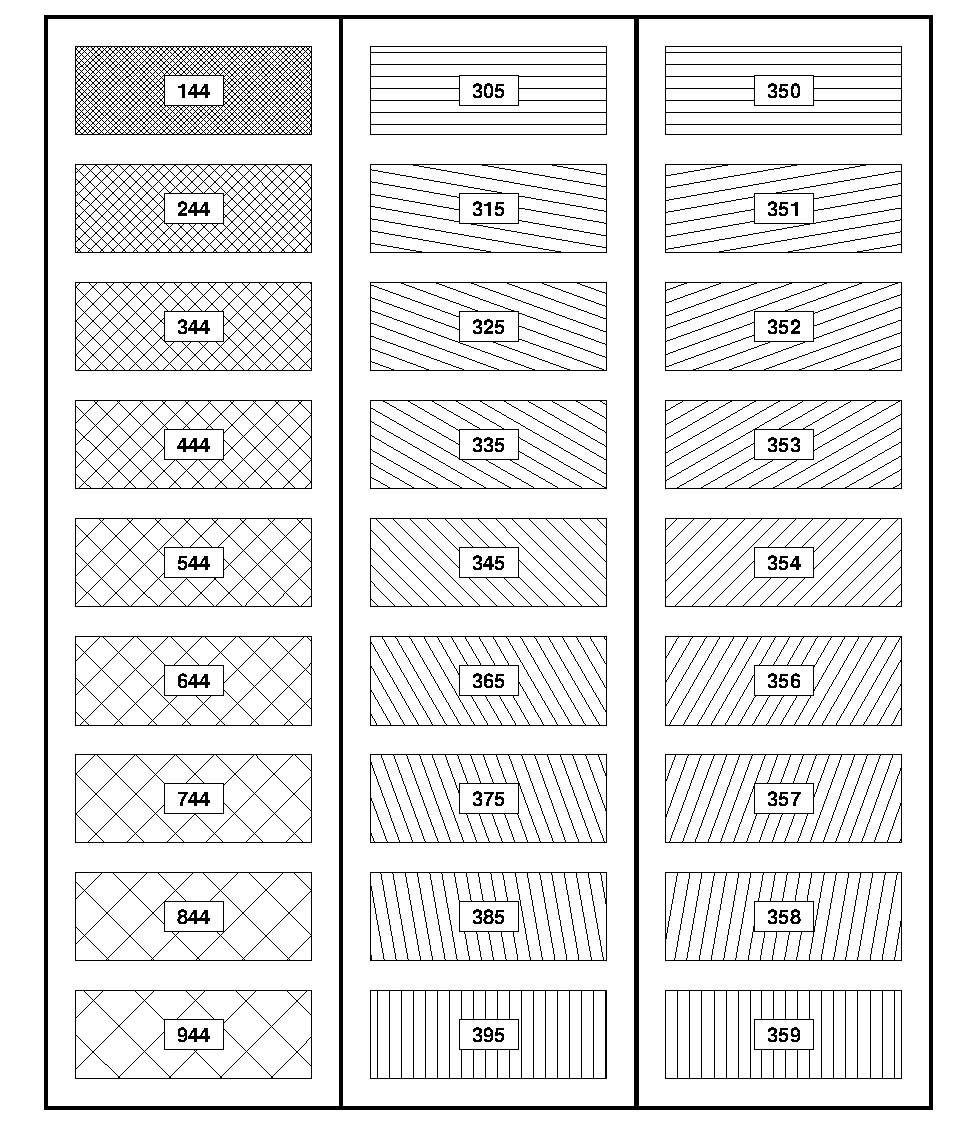
\includegraphics[width=\linewidth]{fasi.eps}
\caption{\HIGZ~portable fill area hatch styles.}
\label{FILL-STY}
\end{figure}
\clearpage
%
\subsection{Line type.}
\index{polyline!type}
\Shubr[GKS]{ISLN}{(LTYPE)}
\Action
This routine sets the line type attribute for use by future invocations of
\Rind{IPL}. All workstations support at least line types 1 through 4
(see figure \ref{LINE-TYPE}). Other line types may be supported. If a requested
line type is not supported on a workstation, line type 1 is used when polylines
are created.
The routine \Rind{IGSET} (see section \ref{IGSET}) can also be used with the
parameter \Sind{LTYP}.
\Pdesc
\begin{DLtt}{1234567}
\item[LTYPE] Line type (positive number).
\begin{DLtt}{123}
\item[1] Solid lines
\item[2] Dashed lines
\item[3] Dotted lines
\item[4] Dashed-dotted lines
\end{DLtt}
\end{DLtt}
\par
Note that line type values are dependent upon the \UGP~used. For the user's
convenience, \HIGZ~defines a number of line types, indicated in the figure
\ref{LINE-TYPE}, which are independent from the basic graphics package used.
%
\subsection{Line width scale factor.}
\index{polyline!width}
\Shubr[GKS]{ISLWSC}{(WIDTH)}
\Action
This routine sets the width of a line for use by future invocations of the
polyline drawing routine \Rind{IPL}. The actual line width is determined by a
nominal line width (workstation-dependent) multiplied by the line width scale
factor. The nominal line width is one pixel on screens. On \PS~printers the
nominal line width is one ``dot''. Therefore the width of a line can vary from
a printer to another depending on the printer definition (300 dots per inch,
400 dots per inch etc.). The figure \ref{LINE-WIDTH} shows some examples of
various line width. The routine \Rind{IGSET} (see section \ref{IGSET}) can also
be used with the parameter \Sind{LWID}.
\Pdesc
\begin{DLtt}{1234567}
\item[WIDTH] Line width scale factor.
\end{DLtt}

\begin{figure}[p]
\begin{center}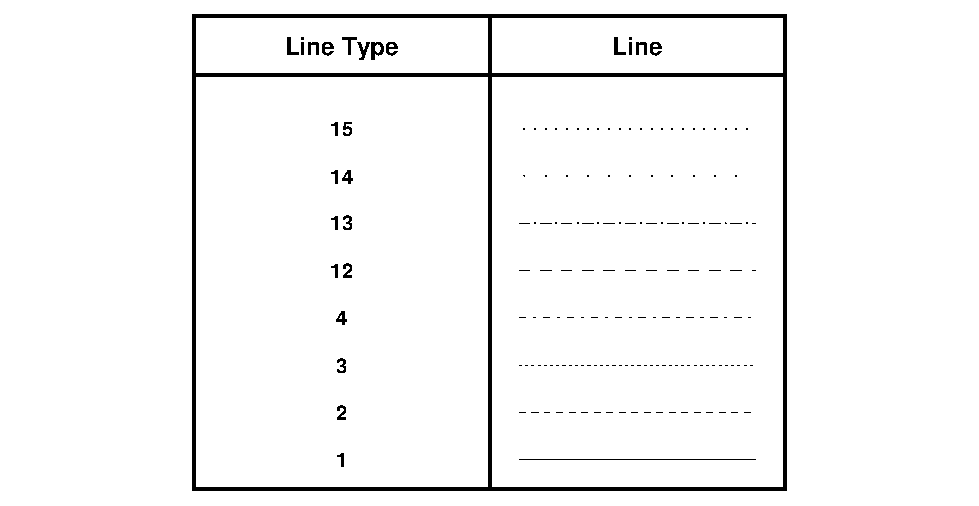
\includegraphics{line.eps}\end{center}
\caption{Line styles available.}
\label{LINE-TYPE}

\bigskip

\begin{center}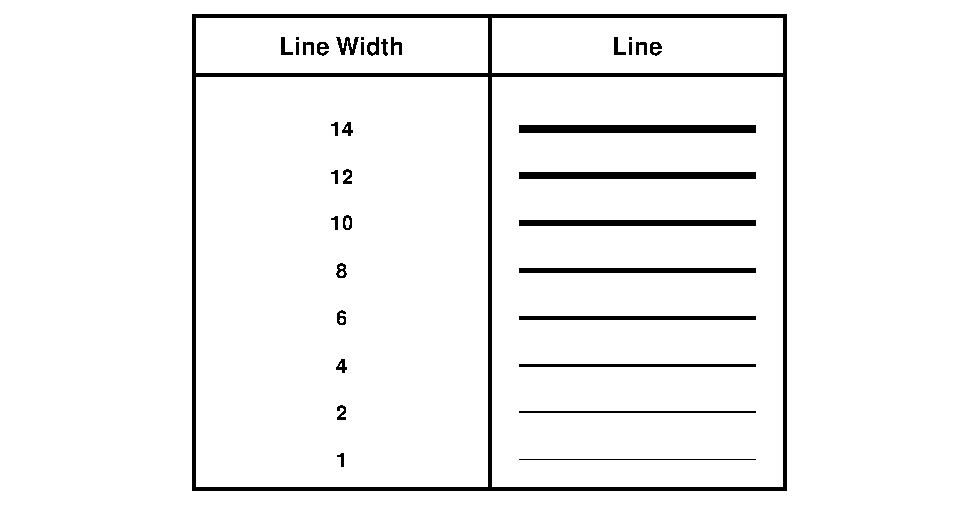
\includegraphics{linew.eps}\end{center}
\caption{Examples of line width.}
\label{LINE-WIDTH}
\end{figure}
\clearpage
%
\subsection{Marker type}
\index{polymarker!type}
\Shubr[GKS]{ISMK}{(MTYPE)}
\Action
This routine sets the marker type attribute for use by future invocations of
\Rind{IPM}. All workstations support at least the marker types 1 through 5
(see below). More marker types may be supported by the \UGP. Marker types 20 to
31 are also defined, according to the figure~\ref{MARKER-TYPE}, and are
independent from the \UGP~used. If a requested marker type is not supported on a
workstation, marker type 1 (a point) is used when polymarkers are created.
The routine \Rind{IGSET} (see section \ref{IGSET}) can also be used with the
parameter \Sind{MTYP}.
\Pdesc
\begin{DLtt}{1234567}
\item[MTYPE] Marker type (positive number)
\begin{DLtt}{123}
\item[1] Point shape ($\cdot$).
\item[2] Plus shape ($+$).
\item[3] Asterisk shape ($\ast$).
\item[4] Circle shape ($\circ$).
\item[5] X shape ($\times$).
\end{DLtt}
\end{DLtt}
%
\subsection{Marker scale factor.}
\index{polymarker!scale factor}
\Shubr[GKS]{ISMKSC}{(SSFM)}
\Action
This routine sets the marker scale factor. This scale factor is applied on
the nominal size of the marker. On all workstation, except \PS{} files, the marker
type 1 is not scalable. The routine \Rind{IGSET} (see section \ref{IGSET}) can
also be used with the parameter \Sind{MSCF}.
\Pdesc
\begin{DLtt}{1234567}
\item[SSFM] Scale factor applied to markers. (\(\geq0.\))
\end{DLtt}

\begin{figure}[p]
\begin{center}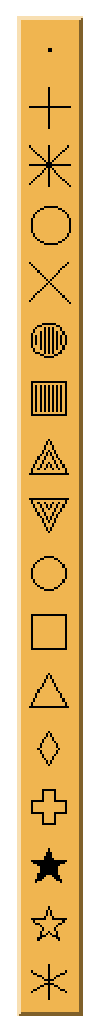
\includegraphics{marker.eps}\end{center}
\caption{\HIGZ~Marker type (20-31).}
\label{MARKER-TYPE}

\bigskip

\begin{center}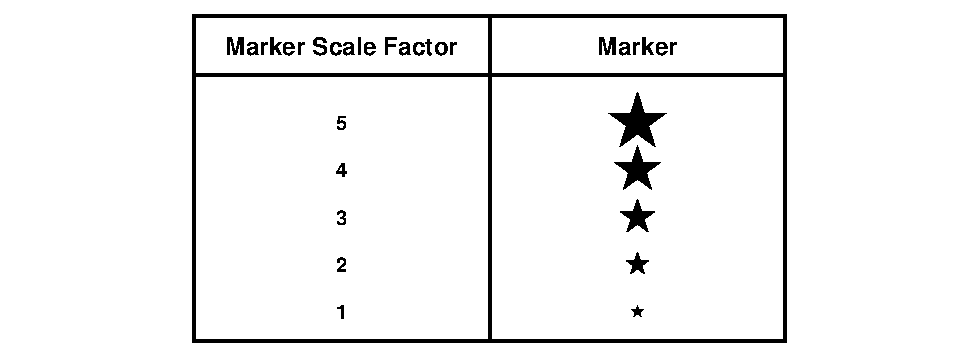
\includegraphics{markersf.eps}\end{center}
\caption{Examples marker scale factor.}
\label{MARKER-SIZE}
\end{figure}
\clearpage
%
\subsection{Text alignment.}
\index{text!alignment}
\Shubr[GKS]{ISTXAL}{(ITXALH,ITXALV)}
\Action
This routine sets the text alignment attribute for use by future invocations
of \Rind{ITX}. Text alignment controls the placement of the character string
with respect to the position specified in the call to \Rind{ITX}. Horizontal
alignment specifies which end of the string (or its geometric center) is
aligned with the point specified in \Rind{ITX}. For a given horizontal
alignment, the vertical alignment controls whether the tops of tall characters
or the bottoms of capital letters line up with the point specified (see figure
\ref{TEXT-ALIGN}). The routine \Rind{IGSET} (see section \ref{IGSET}) can also
be used with the parameter \Sind{TXAL}.
\Pdesc
\begin{DLtt}{1234567}
\item[ITXALH] Horizontal alignment specifier ({\tt0$\leq$ITXALH$\leq$3})
\begin{DLtt}{123}
\item[0] Left end of string at point specified (normal).
\item[1] Same as {\tt 0}.
\item[2] Center of string at point specified.
\item[3] Right end of string at point specified.
\end{DLtt}
\item[ITXALV] Vertical alignment specifier ({\tt0\(\leq\)ITXALV\(\leq\)5})
\begin{DLtt}{123}
\item[0] Base of the characters (normal).
\item[1] Top of tallest characters.
\item[2] Same as {\tt 2}.
\item[3] Middle of tallest characters.
\end{DLtt}
\end{DLtt}
\begin{Fighere}
\begin{center}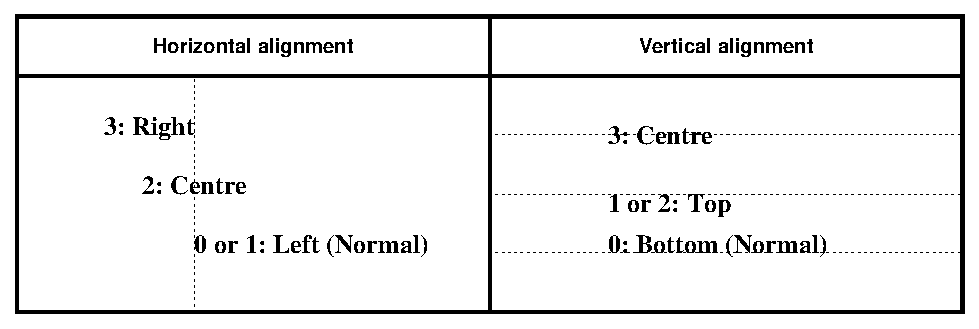
\includegraphics{align.eps}\end{center}
\caption{Text alignment.}
\label{TEXT-ALIGN}
\end{Fighere}
%
\newpage%%%%%%%%%%%%%%%%%%%%%%%%%%%%%%%%%%%%%%%%%%%%%%%%%%%%%%%%%%%%%%%%%%%%%%
\subsection{Character height}
\index{text!character height}
\Shubr[GKS]{ISCHH}{(CHH)}
\Action
This routine sets the character height attribute for use by future invocations
of \Rind{ITX}. The routine \Rind{IGSET} (see section \ref{IGSET}) can also be
used with the parameter \Sind{CHHE}.
\Pdesc
\begin{DLtt}{1234567}
\item[CHH] Character height. The default set by \Rind{IGSSE} is {\tt0.01}. The
           height is given in \WC~and it must be positive.
\end{DLtt}
%
\subsection{Character up vector.}
\index{text!character up vector}
\index{text!angle}
\Shubr[GKS]{ISCHUP}{(RCHUX, RCHUY)}
\Action
This routine sets the ``character up vector'' attribute for use by future
invocations of \Rind{ITX}. The angle of the text can also be specified via the
\Rind{IGSET} routine with the parameter \Sind{TANG}.
\Pdesc
\begin{DLtt}{1234567}
\item[RCHUX] Character up vector in \WC~(x part).
\item[RCHUY] Character up vector in \WC~(y part).
\end{DLtt}
The size of the vector specified is immaterial, but
{\tt CHUX$^2$+CHUY$^2$>1.E-20}.
%
\subsection{Text font and precision.}
\index{text!font and precision}
\Shubr[GKS]{ISTXFP}{(IFONT,IPREC)}
\Action
This routine sets the text font and precision attributes for use by future
invocations of \Rind{ITX}. The text font parameter selects among possible
character shapes, as a roman font, a sans-serif font, etc. The text precision
parameter specifies how closely \HIGZ~(and also the \UGP) must follow the
current size and orientation attributes. String precision is most liberal,
stroke precision is most strict. Character precision is in the middle.
The routine \Rind{IGSET} (see section \ref{IGSET}) can also be used with the
parameter \Sind{TXFP}.
\Pdesc
\begin{DLtt}{1234567}
\item[IFONT] Text font. The value of {\tt IFONT} depends on the \UGP~used.
\item[IPREC] Text precision ({\tt0\(\leq\)IPREC\(\leq\)2}).
\end{DLtt}
Note that font number 0, with precision 2, is always available, independently
from the \UGP~used and allows to access the \Rind{IGTEXT} facilities from
\Rind{ITX}. If a font is not available on a workstation, or it is supported
but not with the requested precision, font 1 is used, with precision 0.

\subsubsection{The \PS~text fonts}
\index{PostScript!fonts}
\index{PostScript!fonts!Times-Italic}
\index{PostScript!fonts!Times-Bold}
\index{PostScript!fonts!Times-BoldItalic}
\index{PostScript!fonts!Helvetica}
\index{PostScript!fonts!Helvetica-Oblique}
\index{PostScript!fonts!Helvetica-Bold}
\index{PostScript!fonts!Helvetica-BoldOblique}
\index{PostScript!fonts!Courier}
\index{PostScript!fonts!Courier-Oblique}
\index{PostScript!fonts!Courier-Bold}
\index{PostScript!fonts!Courier-BoldOblique}
\index{PostScript!fonts!Symbol}
\index{PostScript!fonts!Times-Roman}
\index{PostScript!fonts!ZapfDingbats}
With \PS~work\-sta\-tion types, the text pro\-du\-ced by \Rind{ITX} can be
ge\-ne\-ra\-ted with \PS~fonts. The figure \ref{PS-FONT} shows all the \PS~fonts
avai\-lable on most \PS~prin\-ters. Note that the fonts {\tt -15} to {\tt -24}
are the same than {\tt -1} to {\tt -14}, but they are drawn in hollow mode.

The {\sf ZapfDingbats} font is not available on all \PS~printers. On such
printers \index{PostScript!printers} a reference to this font will produce an
error message. The correspondence between \ASCII~and {\sf ZapfDingbats} font
is given on figures \ref{PSTEXT1} and \ref{PSTEXT2}.
\Rind{IGTEXT} control characters are taken into account. In addition
the character $\sim$ switches to the {\sf ZapfDingbats} character set.
\index{lower case letters}
\index{upper case letters}
\index{Greek letters}
\index{superscript}
\index{subscript}
\index{backspace}
\index{termination character}
\index{special symbols}
\begin{center}
\begin{tabular}{||c|l||c|l||}
\hline
\multicolumn{4}{|c|}{\bf List of escape characters and their meaning}         \\
\hline
 $<$  & go to lower case (optional)      & $>$  & go to upper case (optional) \\
\hline
 \lsb & go to greek (Roman = default)    & \rsb & end of greek                \\
\hline
 "    & go to special symbols            & \#   & end of special symbols      \\
\hline
$\sim$ & go to ZapfDingbats              & \#   & end of ZapfDingbats         \\
\hline
$\uparrow$  & go to superscript          & ?    & go to subscript             \\
\hline
 !    & go to normal level of script     & \&   & backspace one character     \\
\hline
 \$   & termination character (optional) &  @   & escape                      \\
\hline
\end{tabular}
\end{center}
\par
The \PS~fonts can be used with precision {\tt 0} or precision {\tt 1}. On the 
screen, a \PS~font used with precision {\tt 1} appears like the \Rind{IGTEXT} 
characters, with precision 0 its appears as hardware character (\X11{} fonts).
In both cases the \PS~file is the same. Note that characters can also be 
entered directly in lower or upper case instead of using the escape characters
{\tt <} and {\tt >}. The escape characters can be themselves escaped with the 
{\tt @} sign i.e: {\tt '@<'} produce a {\tt <} symbol.

\clearpage

\begin{XMPt}{Example of \PS~ text (result in figure \ref{PSEX1})}
      program psex1
      call start('psex1',16.,5.)
      call igset('LWID',6.)
      call igbox(0.,16.,0.,5.)
      call igset('CHHE',0.5)
      call igset('TXAL',3.)
      call igset('TXFP',-130.)
*
      call itx(3.,4.,'K\bs{}355nstler in den gr\bs{}345\bs{}373ten st\bs{}311dten')
      call itx(3.,3.,'\bs{}253\bs{}265 l''\bs{}372uvre on conna\bs{}333t l''artisan\bs{}273')
      call itx(3.,2.,'\bs{}(proverbe fran\bs{}321ais\bs{}).')
      call itx(3.,1.,
     + '\bs{}252\bs{}241Ma\bs{}337ana\bs{}41 \bs{}322ag&\bs{}306!das&\bs{}313!\bs{}272, '
     + //'dit l''\bs{}323l\bs{}325ve.')
*
      call finish
      end
\end{XMPt}

\begin{Fighere}
\begin{center}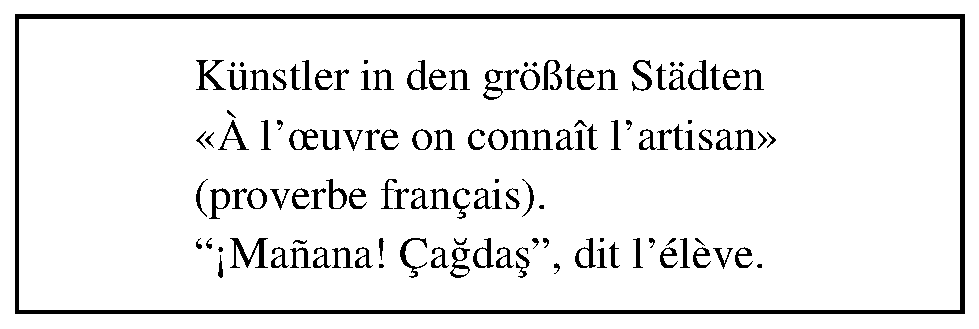
\includegraphics{psex1.eps}\end{center}
\caption{\PS~fonts usage (1).}
\label{PSEX1}
\end{Fighere}

\clearpage

\begin{XMPt}{Example of \PS~ text and maths (result in figure \ref{PSEX2})}
      program psex2
      call start('psex2',16.,5.)
      call igset('LWID',6.)
      call igbox(0.,16.,0.,5.)
      call igset('CHHE',0.5)
      call igset('TXAL',23.)
      call igset('TXFP',-130.)
*
      call itx(8.,4.,
     +'e^+!e^-! "5# Z^o! "5# ll&^-!, qq&^\bs{}261!')
      call itx(8.,3.,
     +'| a&^[\bs{}256]! \bs{}267 b&^[\bs{}256]! | = [\bs{}345] a^i?jk!+b^kj?i')
      call itx(8.,2.,
     + 'i ("d#?[m!y]&^\bs{}261![g^m]! + m [y]&^\bs{}261! ) = 0'//
     + '" r# (~r# + m^2!) [y] = 0')
      call itx(8.,1.,
     + 'L?em! = e J^[m]?em! A?[m]! , J^[m]?em!=l&^\bs{}261![ g?m]!l , '//
     + 'M^j?i! = [\bs{}345&?a]! A?[a! t^a]j?i! ')
*
      call finish
      end
\end{XMPt}

\begin{Fighere}
\begin{center}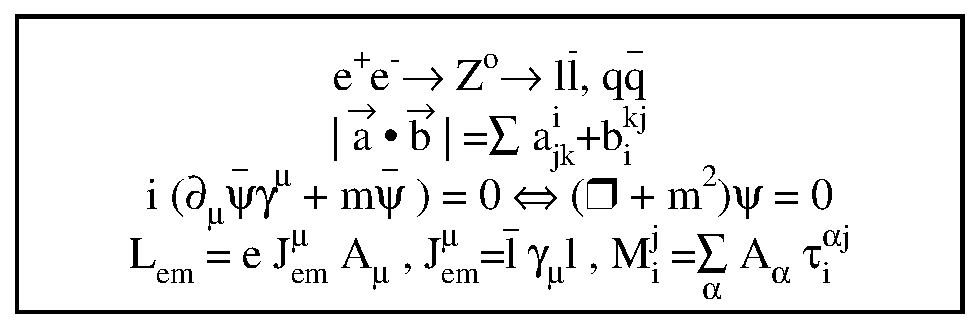
\includegraphics{psex2.eps}\end{center}
\caption{\PS~fonts usage (2).}
\label{PSEX2}
\end{Fighere}

\clearpage

\begin{figure}[p]
\includegraphics[width=\linewidth]{psfont.eps}
\caption{\PS~ text fonts.}
\label{PS-FONT}
\end{figure}

\begin{figure}[p]
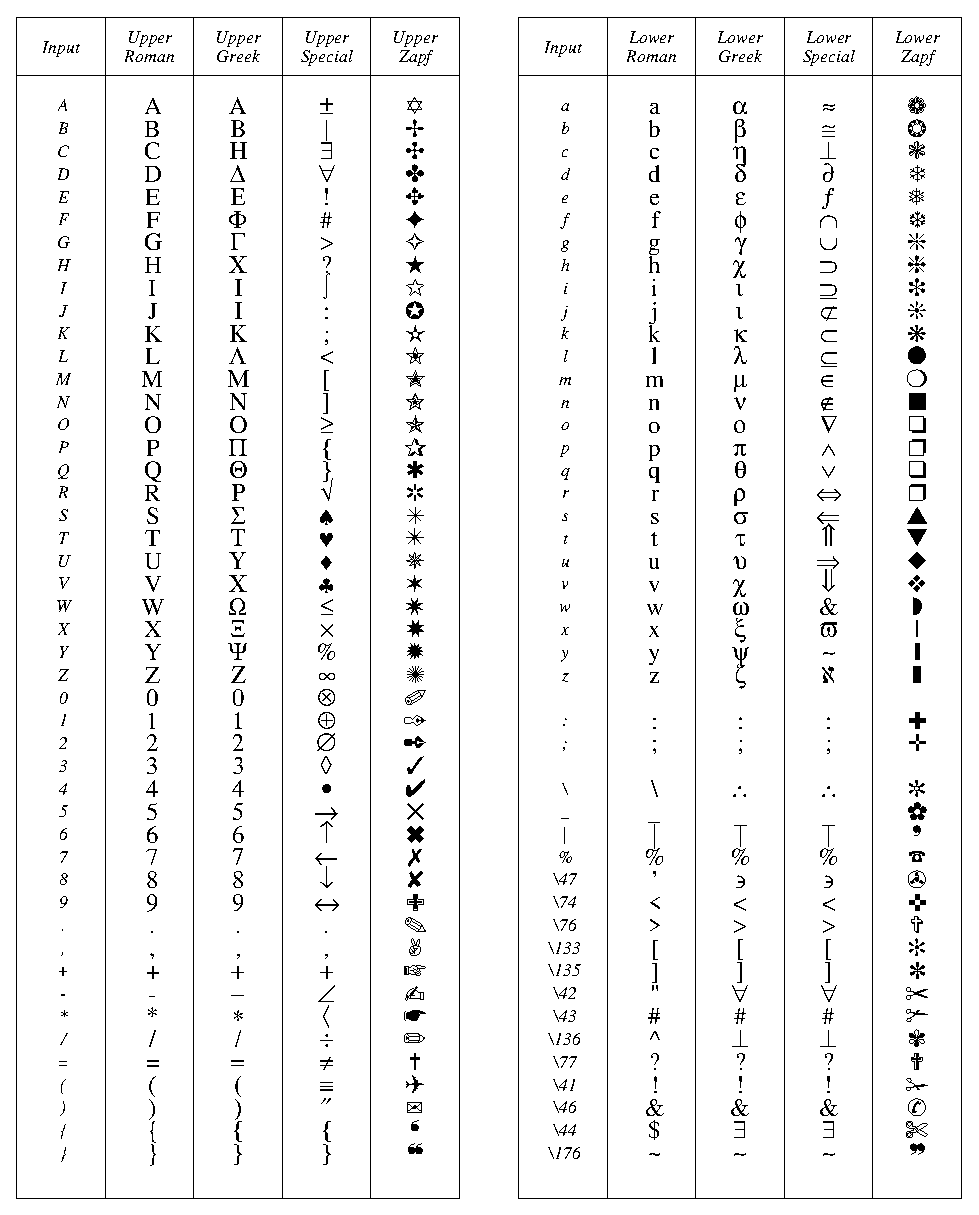
\includegraphics[width=\linewidth]{pstext1.eps}
\caption{\PS~ characters (1).}
\label{PSTEXT1}
\end{figure}

\begin{figure}[p]
\begin{center}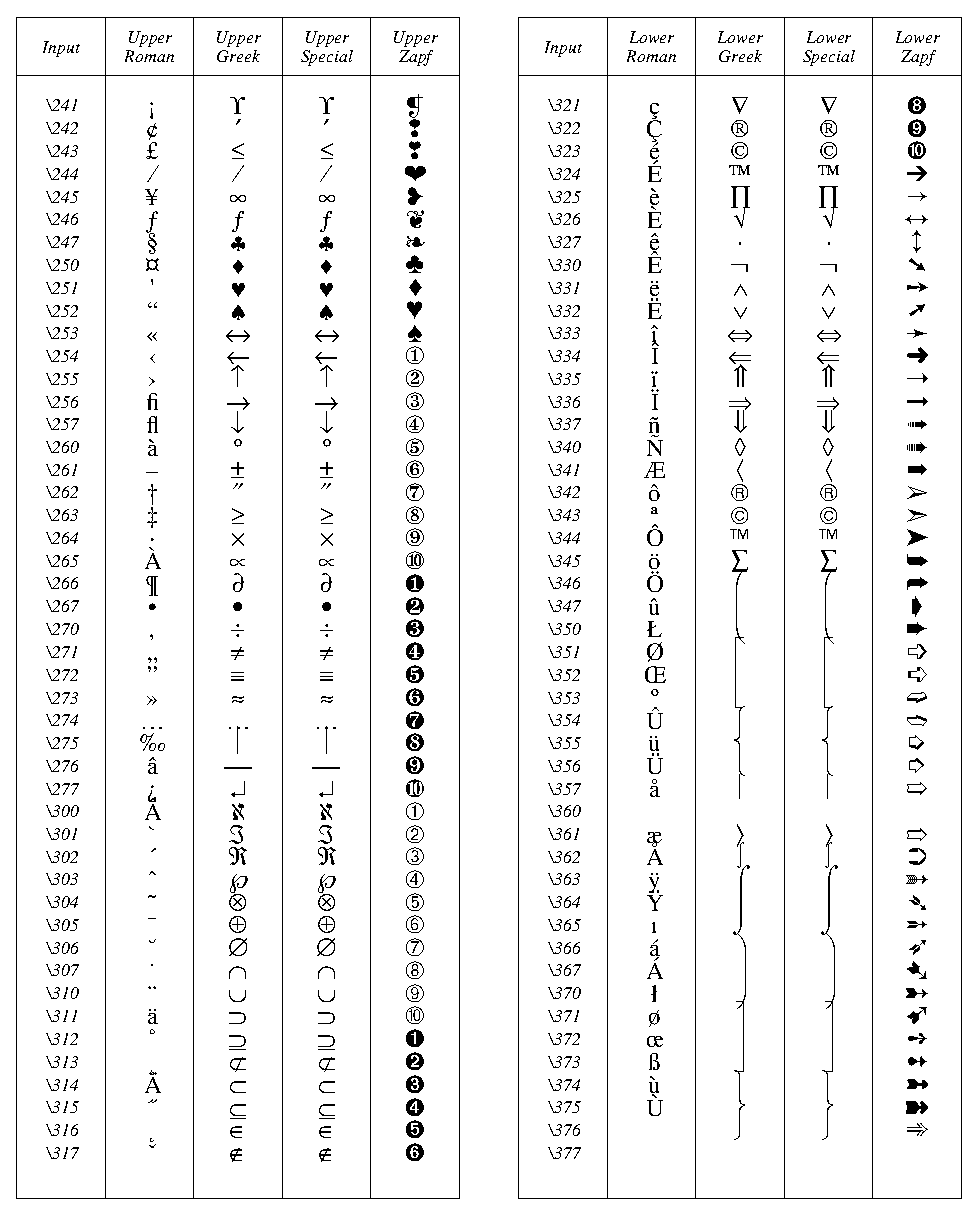
\includegraphics[height=19cm]{pstext2.eps}\end{center}
\caption{\PS~ characters (2).}
\label{PSTEXT2}
\end{figure}
\clearpage
\mbox{}
\clearpage

